%%%%%%%%%%%%%%%%%%%%%%%
% Comp 170, Fall 2019
% Homework 10
% Author: Vladimir Hugec
%%%%%%%%%%%%%%%%%%%%%%%

% This portion of the LaTeX document are configuration 
% You can see it as all the #includes in C++
\documentclass[12pt]{article}

\usepackage{epsfig}
\usepackage{amsmath}
\usepackage{amsthm}
\usepackage{listings}
\usepackage{graphicx}
\usepackage{tikz}

\newtheorem{lemma}{Lemma}
\newtheorem{theorem}{Theorem}

\usepackage{titlesec}
\titleformat{\section}
{\normalfont\Large\bfseries}{Question~\thesection:}{1em}{}

\newlength{\toppush}
\setlength{\toppush}{2\headheight}
\addtolength{\toppush}{\headsep}

\def\subjnum{Comp 170}
\def\subjname{Computation Theory}

\def\doheading#1#2#3{\vfill\eject\vspace*{-\toppush}%
  \vbox{\hbox to\textwidth{{\bf} \subjnum: \subjname \hfil Vladimir Hugec}%
    \hbox to\textwidth{{\bf} Tufts University, Fall 2019 \hfil#3\strut}%
    \hrule}}


\newcommand{\htitle}[1]{\vspace*{1.25ex plus 1ex minus 0ex}%
\begin{center}
{\large\bf #1}
\end{center}} 


%%%%%%%%%%%%%%%%%%%%%%%%%%%%%%%%%%%%%%%%%%%%%%%%%%%%%%%%%%%%%%%%%%%
% BEGIN DOCUMENT
%%%%%%%%%%%%%%%%%%%%%%%%%%%%%%%%%%%%%%%%%%%%%%%%%%%%%%%%%%%%%%%%%%%
\begin{document}
\doheading{2}{title}{Homework 10}

\section{}

\subsection{A}

A polynomial time algorithm $A$ for $COLOR_{1}$ operates as folllows. 
$\newline$

$A = $ "On input $\langle G \rangle $ where $G$ is a graph that can be colored with one color:
$\newline \indent$ 1. Select an arbitrary node $x$ to begin and color it one color.
$\newline \indent$ 2. For each neighbor of $x$, $y_{1}, y_{2}, ... y_{n}$ color them the same color as $x$.
$\newline \indent$ 3. Repeat step 2. for each neighbor of $y_{1}, y_{2}, ..., y_{n}$.
$\newline \indent$ 4. Continue until all nodes in $G$ are colored. "

$\newline$
NOTE: This is just a BFS

\subsection{B}

A polynomial time algorithm $B$ for $COLOR_{2}$ operates as folllows. 
$\newline$

$B = $ "On input $\langle G \rangle $ where $G$ is a graph that can be colored with two colors:
$\newline \indent$ 1. Select an arbitrary node $x$ to begin and color it one color.
$\newline \indent$ 2. For each neighbor of $x$, $y_{1}, y_{2}, ... y_{n}$ color them with the other color.
$\newline \indent$ 3. Repeat step 2. for each neighbor of $y_{1}, y_{2}, ..., y_{n}$, coloring them the $\newline \indent $ opposite color as their predecessors.
$\newline \indent$ 4. Continue until all nodes in $G$ are colored. "
$\newline \indent$ 5. Verify that all for nodes that are connected by an edge, then those $\newline \indent$ vertices are assigned different colors. If test passes then Graph is $\newline \indent$ 2-colorable.

$\newline$ NOTE: As above, just a BFS

\pagebreak

\section{}

To show that $COLOR_{k}$ is polynomial time reducible to $COLOR_{k+1}$, assume we have a graph $G$ that is $k$-colored. Now we create a new node of an arbitrary color that is not present in $G$. Now suppose we duplicate $G$ as $G'$ with the caveat that the new node we created will be attached to every other original node in $G$. This way we know that since $G$ is $k$-colored, then $G'$ must be $k+1$-colored. And similarly in reverse, if we know $G'$ is $k+1$-colored, since we node our arbitrarily colored node is not present in $G$ but $G$ is exactly the same otherwise to $G'$, we know $G$ must be $k$-colorable. And so $COLOR_{k} \leq_{P} COLOR_{k+1}$.

Since we know that $COLOR_{1} \in P$, $COLOR_{2} \in P$ and $COLOR_{3}$ is NP-complete. $\forall k \geq 3$ we can reduce $COLOR_{k}$ to $COLOR_{k+1}$ and so we know that $\forall k \geq 3$, $COLOR_{k}$ must be NP-complete.

\pagebreak

\section{}

\subsection{A}

The certificate would be the 3 sets of vertices.

\subsection{B}

To show that $G \in COLOR_{3} \iff G' \in FOREST_{3}$. Assume that $G$ is $3$-colorable. We know that since $G$ is $3$-colorable, a particular node can only be connected to a maximum of $2$ other nodes. Any more than that and the graph is not $3$ colorable. Assume we have a simple graph, $G$, that is $3$-colorable as shown below:

\begin{center}
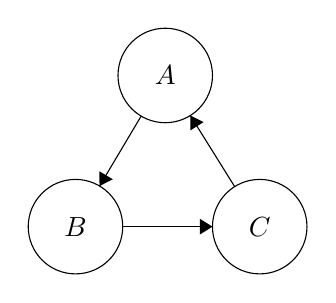
\begin{tikzpicture}[scale=0.2]
\tikzstyle{every node}+=[inner sep=0pt]
\draw [black] (37.9,-4.5) circle (3);
\draw (37.9,-4.5) node {$A$};
\draw [black] (32.2,-14.1) circle (3);
\draw (32.2,-14.1) node {$B$};
\draw [black] (43.9,-14.1) circle (3);
\draw (43.9,-14.1) node {$C$};
\draw [black] (36.37,-7.08) -- (33.73,-11.52);
\fill [black] (33.73,-11.52) -- (34.57,-11.09) -- (33.71,-10.58);
\draw [black] (35.2,-14.1) -- (40.9,-14.1);
\fill [black] (40.9,-14.1) -- (40.1,-13.6) -- (40.1,-14.6);
\draw [black] (42.31,-11.56) -- (39.49,-7.04);
\fill [black] (39.49,-7.04) -- (39.49,-7.99) -- (40.34,-7.46);
\end{tikzpicture}
\end{center}






Now, adding in $v_{1}, v_{2}, v_{3}$ and connecting it to every other node in the graph including themselves:

\begin{center}
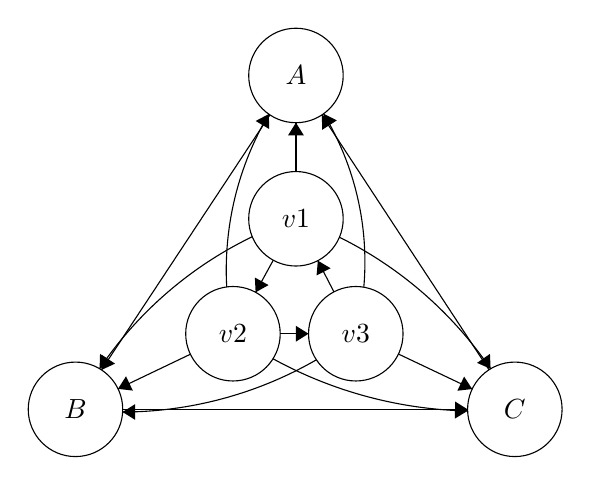
\begin{tikzpicture}[scale=0.2]
\tikzstyle{every node}+=[inner sep=0pt]
\draw [black] (37.9,-4.5) circle (3);
\draw (37.9,-4.5) node {$A$};
\draw [black] (23.9,-25.7) circle (3);
\draw (23.9,-25.7) node {$B$};
\draw [black] (51.8,-25.7) circle (3);
\draw (51.8,-25.7) node {$C$};
\draw [black] (37.9,-13.6) circle (3);
\draw (37.9,-13.6) node {$v1$};
\draw [black] (33.9,-20.9) circle (3);
\draw (33.9,-20.9) node {$v2$};
\draw [black] (41.7,-20.9) circle (3);
\draw (41.7,-20.9) node {$v3$};
\draw [black] (36.25,-7) -- (25.55,-23.2);
\fill [black] (25.55,-23.2) -- (26.41,-22.8) -- (25.58,-22.25);
\draw [black] (26.9,-25.7) -- (48.8,-25.7);
\fill [black] (48.8,-25.7) -- (48,-25.2) -- (48,-26.2);
\draw [black] (50.16,-23.19) -- (39.54,-7.01);
\fill [black] (39.54,-7.01) -- (39.57,-7.95) -- (40.4,-7.4);
\draw [black] (36.46,-16.23) -- (35.34,-18.27);
\fill [black] (35.34,-18.27) -- (36.16,-17.81) -- (35.29,-17.33);
\draw [black] (36.9,-20.9) -- (38.7,-20.9);
\fill [black] (38.7,-20.9) -- (37.9,-20.4) -- (37.9,-21.4);
\draw [black] (40.31,-18.24) -- (39.29,-16.26);
\fill [black] (39.29,-16.26) -- (39.21,-17.2) -- (40.1,-16.74);
\draw [black] (37.9,-10.6) -- (37.9,-7.5);
\fill [black] (37.9,-7.5) -- (37.4,-8.3) -- (38.4,-8.3);
\draw [black] (31.2,-22.2) -- (26.6,-24.4);
\fill [black] (26.6,-24.4) -- (27.54,-24.51) -- (27.11,-23.6);
\draw [black] (44.41,-22.19) -- (49.09,-24.41);
\fill [black] (49.09,-24.41) -- (48.58,-23.62) -- (48.15,-24.52);
\draw [black] (33.504,-17.929) arc (-176.83017:-210.58375:19.455);
\fill [black] (36.18,-6.95) -- (35.34,-7.39) -- (36.2,-7.9);
\draw [black] (39.656,-6.929) arc (31.14182:-5.05054:18.206);
\fill [black] (39.66,-6.93) -- (39.64,-7.87) -- (40.5,-7.35);
\draw [black] (48.803,-25.803) arc (-91.23854:-118.78362:26.876);
\fill [black] (48.8,-25.8) -- (48.01,-25.29) -- (47.99,-26.29);
\draw [black] (39.199,-22.554) arc (-59.99643:-89.82043:24.764);
\fill [black] (26.89,-25.87) -- (27.69,-26.37) -- (27.69,-25.37);
\draw [black] (25.428,-23.121) arc (145.87653:115.79625:24.699);
\fill [black] (25.43,-23.12) -- (26.29,-22.74) -- (25.46,-22.18);
\draw [black] (40.66,-14.771) arc (63.60585:34.31477:25.17);
\fill [black] (50.26,-23.13) -- (50.22,-22.18) -- (49.4,-22.75);
\end{tikzpicture}
\end{center}

We can see that the set of $3$ subgraphs is $\lbrace A, v_{1} \rbrace$, $\lbrace B, v_{2} \rbrace$, $\lbrace C, v_{3} \rbrace$. Adding in more nodes to $G$, we notice that it is always possible to split the new $G'$ into $3$ subgraphs. If we add node $D$ connected to each $A, B$, the subgraphs would become $\lbrace A, v_{1}, C \rbrace$, $\lbrace B, v_{1}, v_{2} \rbrace$, $\lbrace D \rbrace$. If we add node $E$ connected to each $C, D$, the subgraphs would become $\lbrace A, v_{1}, C \rbrace$, $\lbrace B, v_{1}, v_{2} \rbrace$, $\lbrace D, E \rbrace$. The pattern continues. And so we know that if $G$ is $3$ colorable then $G' \in FOREST_{3}$. Similarly in reverse, since we know $G' \in FOREST_{3}$, we know that $v_{1}, v_{2}, v_{3}$ are the only nodes that violate the connection to a max of two other nodes rule. So if those nodes are removed then it must be possible to $3$-color the resultant graph.





\enddocument
 
%%%%%%%%%%%%%%%%%%%%%%%%%%%%%%%%%%%%%%%%%%%%%%%%%%%%%%%%%%%%%%%%%%%%%%

